\chapter{Desarrollo}
\section{Análisis}

El análisis de un filtro digital es el proceso de determinar la respuesta de un filtro ante una dada excitación. El presente informe tiene como objetivo documentar los pasos que serán necesarios para realizar el diseño de un filtro digital a partir de un prototipo con determinadas características o especificaciones.

En el contexto de la problemática comentada en el capítulo anterior, disponemos de 10 señales a analizar las cuales se corresponden con los digitos del 0 al 9. De esto concluímos que se necesitan 10 bandas de paso para filtrar las 10 señales. Dada la cercanía de las frencuencias centrales por dígito (ver Cuadro \ref{tab:combinacion_tonos}) se propone un \gls{ab} de 20Hz por frecuencia. De esta forma la distribución bandas de paso queda determinado por el Cuadro \ref{tab:anchos_de_banda}.

Los límites de frecuencia de cada \gls{ab} corresponden a los puntos de media potencia (0.707) del valor máximo de
transferencia. Además, establecemos como criterio de diseño que debe atenuar a 20dB en la banda de transición o paso.

\begin{table}[H]
  \centering
  \begin{tabular}{|Sc|Sc|Sc|Sc|}
    \hline
    \textbf{Digito} & \textbf{$f_{c1}$} & \textbf{$f_0$} & \textbf{$f_{c2}$} \\
    \hline
    1               & 1896              & 1906           & 1916              \\ \hline
    4               & 1969              & 1979           & 1989              \\ \hline
    2               & 2023              & 2033           & 2043              \\ \hline
    7               & 2051              & 2061           & 2071              \\ \hline
    5               & 2096              & 2106           & 2116              \\ \hline
    3               & 2164              & 2174           & 2184              \\ \hline
    8               & 2178              & 2188           & 2198              \\ \hline
    6               & 2237              & 2247           & 2257              \\ \hline
    0               & 2267              & 2277           & 2287              \\ \hline
    9               & 2319              & 2329           & 2339              \\ \hline
  \end{tabular}
  \caption{Distribución de bandas de paso (medido en [Hz])}
  \label{tab:anchos_de_banda}
\end{table}

\section{Diseño}
Para el desarrollo de los filtros pasa banda usaremos el método directo con un filtro prototipo pasabajos Butterworth.

\subsection*{Método Directo}
El método directo, también conocido como método de diseño de coeficientes, es uno de los métodos más simples y directos para diseñar filtros digitales. Este método se basa en la especificación directa de los coeficientes del filtro en función de los parámetros deseados, como la respuesta de frecuencia, la \gls{fc} y las características de atenuación.

\subsection*{Filtro Butterworth}
El filtro Butterworth es un tipo de filtro digital diseñado utilizando la aproximación de Butterworth, que es una de las aproximaciones clásicas para la respuesta de frecuencia de filtros analógicos y digitales. Se caracteriza por tener una respuesta en frecuencia lo más plana y suave posible en la banda de paso, lo que significa que atenúa las frecuencias no deseadas de manera gradual y sin oscilaciones abruptas.

El filtro de Butterworth más típico es el filtro pasa bajo de primer orden, el cual puede ser modificado a un filtro pasa alto o añadir en serie otros formando un filtro pasa banda o elimina banda y filtros de mayores órdenes.

\subsection*{Consideraciones}
Como podemos observar en el Cuadro \ref{tab:anchos_de_banda} la región espectral más comprometida es la que corresponde a los digitos 3 y 8 debido su cercanía en frecuencia, por lo que procederemos a calcular el filtro para el dígito 8. Luego, lo usaremos como base para los demás filtros, ya que si cumple las especificaciones para la región entre frecuencias más cercanas, se cumplirá en las demás frecuencias. Realizamos el cálculo del orden del filtro Butterworth prototipo pasa-bajo. El filtro pasa-banda será el doble del orden calculado para el prototipo pasa-bajos.

\section{Especificaciones}
Definimos la \gls{fs} apropiada utilizando el Teorema de Nyquist-Shannon, teniendo en cuenta la banda de frecuencias de interés. La frencuencia máxima del sistema es 2339Hz (banda lateral superior del dígito 9). Entonces el cálculo de \gls{fs} está dado por la siguiente expresión:

\begin{equation}
  f_s \geq 2f_{MAX} = 2 \times 2339 \mathrm{[Hz]} = 4678 \mathrm{[Hz]}
\end{equation}

Por cuestiones de diseño tomamos $f_s = 5000[Hz]$. Además también debemos establecer la \gls{fa}, la cual será 4[Hz] mayor que \gls{fc}. Todos los datos necesarios para el diseño del filtro pasa bajos se detalla en el Cuadro \ref{tab:caracteristicas_filtro_pb}.

\begin{table}[H]
  \centering
  \begin{tabular}{|Sc|Sc|}
    \hline
    \textbf{Magnitud} & \textbf{Valor} \\
    \hline
    $f_0$             & 2188[Hz]       \\ \hline
    \gls{fc}          & 2198[Hz]       \\ \hline
    \gls{fa}          & 2022[Hz]       \\ \hline
    \gls{fs}          & 5000[Hz]       \\ \hline
    Atenuación        & 10[dB]         \\ \hline
  \end{tabular}
  \caption{Características de prototipo de filtro pasa bajos}
  \label{tab:caracteristicas_filtro_pb}
\end{table}

Ahora necesitamos obtener el orden ($n$) del filtro. A partir de la Ecuación \ref{eq:atenuacion_db}, podemos despejar $n$ y obtenemos la Ecuación \ref{eq:orden_filtro}. Para poder encontrar el valor de $n$ primero debemos convertir las frecuencias digitales a analógicas, cuyos resultados son obtenidos de las Ecuanciones \ref{eq:omega_a} e \ref{eq:omega_c}.

\begin{equation}
  \omega_{aA} = 2 f_s \tan \frac{2\pi f_a}{2f_s} = 52066,281\ \mathrm{[rad / s]}
  \label{eq:omega_a}
\end{equation}

\begin{equation}
  \omega_{cA} = 2 f_s \tan \frac{2\pi f_c}{2f_s} = 52782,106\ \mathrm{[rad / s]}
  \label{eq:omega_c}
\end{equation}

\begin{equation}
  A_\mathrm{dB} = 10 \log \left[1 + \left(\frac{\omega_{aA}}{\omega_{cA}}\right)^{2n}\right]
  \label{eq:atenuacion_db}
\end{equation}

\begin{equation}
  n = \frac{1}{2} \frac{\log \left(10^{\frac{A_{\mathrm{dB}}}{10}}-1 \right)}{\log \left( \frac{\omega_{cA}}{\omega_{aA}} \right)} = 80,457 \approx 81
  \label{eq:orden_filtro}
\end{equation}

Como se puede obervar en el resultado de la Ecuación \ref{eq:orden_filtro}, el orden es de aproximadamente 81 (porque tiene que ser un número entero positivo). Dado el alto orden que tiene este filtro, el cálculo analítico de los valores se hace sumamente complejo, debido a este problema procederemos a realizar de manera ilustrativa el cálculo para un filtro de \textbf{orden 2}.

\section{Prototipo}
Para el desarrollo analítico del prototipo consideraremos un filtro pasa-bajos de orden 2 (justificado en la sección anterior). Las frecuencias incolucradas se describen en el Cuadro \ref{tab:caracteristicas_filtro_pb}. Como se trata un filtro Butterworth, los polos estables se encontrarán distribuidos sobre el círculo de Butterworth (circulo unitario). Aquellos valores que se encuentren por fuera del mismo, serán los polos inestables. Para este análisis solo consideraremos los estables. Por otro lado, obtendremos los ceros
ubicados en z = -1 como se muestra en la Figura \ref{fig:circulo_butterworth}.

\begin{figure}[ht]
  \centering
  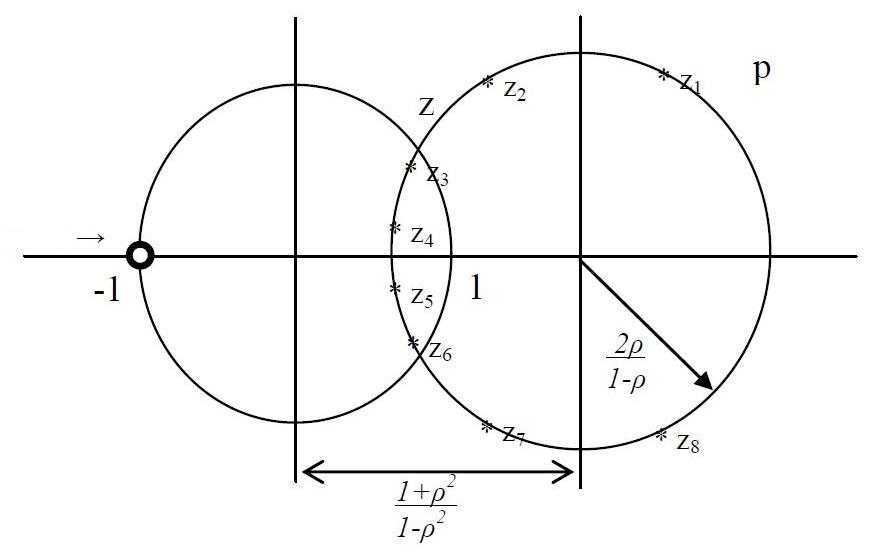
\includegraphics[width=400pt]{images/circulo_butterworth.png}
  \caption{Diagrama de Polos y Ceros}
  \label{fig:circulo_butterworth}
\end{figure}

Para obtener los polos correspondientes al plano z utilizamos la función transferencia, de ella obtenemos la ecuación para obtener los polos (usando la Ecuación \ref{eq:transferencia_u} para obtener las partes reales, y la Ecuación \ref{eq:transferencia_v} para las partes imaginarias).

\begin{equation}
  u_m = \frac
  {1-\tan^2\left(\frac{\omega_cT}{2}\right)}
  {1-2\tan\left(\frac{\omega_cT}{2}\right)\cos\left(\frac{2m+1}{2n}\pi\right)+\tan^2\left(\frac{\omega_cT}{2}\right)}
  \label{eq:transferencia_u}
\end{equation}

\begin{equation}
  v_m = \frac
  {2 \tan\left(\frac{\omega_cT}{2}\right) \sin\left(\frac{2m+1}{2n}\pi\right)}
  {1 - 2 \tan\left(\frac{\omega_cT}{2}\right) \cos\left(\frac{2m+1}{2n}\pi\right) + \tan^2\left(\frac{\omega_cT}{2}\right)}
  \label{eq:transferencia_v}
\end{equation}

\begin{table}[H]
  \centering
  \begin{tabular}{|Sc|Sc|Sc|Sc|Sc|}
    \hline
    \textbf{$m$} & \textbf{$u_m$} & \textbf{$v_m$} & \textbf{Modulo} & \textbf{Argumento} \\
    \hline
    0            & -1,259         & 0,355i         & 1,308           & 2,867              \\ \hline
    1            & -0,736         & 0,208i         & 0,765           & 2,866              \\ \hline
    2            & -0,736         & -0,208i        & 0,765           & -2,866             \\ \hline
    3            & -1,259         & -0,355i        & 1,308           & -2,867             \\ \hline
  \end{tabular}
  \caption{Polos del filtro prototipo}
  \label{tab:polos_resultantes}
\end{table}

Luego para $m=0,1,..., 2n-1$, se optienen 4 polos (ver Cuadro \ref{tab:polos_resultantes}). Del resultado, se puede ver que los polos 0 y 3 se encuentran fuera del círculo unitario, entonces vamos a considerar los polos 1 y 2 para armar la función transferencia del filtro prototipo.

\begin{align}
  H(\textrm{z}) & = \frac{(\textrm{z}-1)^2}{(\textrm{z}-p_1)(\textrm{z}-p_2)}                            \\
  H(\textrm{z}) & = \frac{\textrm{z}^2 + 2\textrm{z} + 1}{\textrm{z}^2 - 2u_1\textrm{z} + u_1^2 + v_1^2} \\
  H(\textrm{z}) & = \frac{\textrm{z}^2 + 2\textrm{z} + 1}{\textrm{z}^2 + 1,472\textrm{z} + 0.585}
\end{align}

Para trabajar en el plano de $\textrm{z}^{-1}$ se multiplica y divide la expresión por $\textrm{z}^{-2}$. Luego obtenemos la Ecuación \ref{eq:funcion_transferencia_z_1} la cual nos indica los coeficientes de la función transferencia.

\begin{equation}
  H(\textrm{z}^{-1}) = \frac
  {1 + 2\textrm{z}^{-1} + \textrm{z}^{-2}}
  {1 + 1,472\textrm{z}^{-1} + 0.585\textrm{z}^{-2}}
  \label{eq:funcion_transferencia_z_1}
\end{equation}

A partir de los coeficientes del polinomio anterior podemos graficar respuesta en frecuencia del filtro utilizando el Código \ref{code:respuesta_freq} en MATLAB. La función que calcula la respuesta en frecuencia es: \lstinline{freqz (N,D)}, donde \lstinline{N} son los coeficientes del numerador, y \lstinline{D} son los coeficientes del denominador. El resultado se puede apreciar en la Figura \ref{fig:respuesta_frecuencia_filtro}.

\lstinputlisting[
  language=Octave,
  caption={Graficar respuesta en frecuencia},
  label={code:respuesta_freq}
]{matlab/respuesta_en_frecuencia.m}

\begin{figure}[H]
  \centering
  
\includegraphics[width=150pt]{images/placeholder.png}
  \caption{Respuesta en frecuencia del filtro}
  \label{fig:respuesta_frecuencia_filtro}
\end{figure}